
{
\rowcolors{1}{ColorAlternatedRow}{}
\newlength{\maximheight} \setlength{\maximheight}{2cm}
\setlength\extrarowheight{4pt}
    
\begin{tabularx}{\textwidth}{%
  >{\setlength{\hsize}{.20\hsize}\raggedright\arraybackslash}X%
  >{\setlength{\hsize}{.25\hsize}}X%
  >{\setlength{\hsize}{.15\hsize}\raggedright\arraybackslash}X%
  >{\setlength{\hsize}{.15\hsize}\raggedright\arraybackslash}X%
  >{\setlength{\hsize}{.10\hsize}\raggedright\arraybackslash}X%
  >{\setlength{\hsize}{.20\hsize}\centering\arraybackslash}X%
}%
%\caption{Comparison of UWB radar development kits}\label{tab:devkits}

\hiderowcolors
\toprule
    Product &
    Note &
    $f_C$, $\Delta f$ &
    Antennas &
    DK Price &
    Picture \\
    \midrule
\endhead

\midrule
\multicolumn{6}{r}{Continued on next page} \\
\endfoot

\bottomrule
\endlastfoot
\showrowcolors

Omniradar RIC60A\footnote{\url{https://www.omniradar.com/products/}} &
High bandwidth. Presentation at SoC 2015 \cite{Brouwer2015} &
\SI{60}{GHz}, \SI{7}{GHz} &
On-chip, 1~Tx,~2~Rx &
\$4000 &
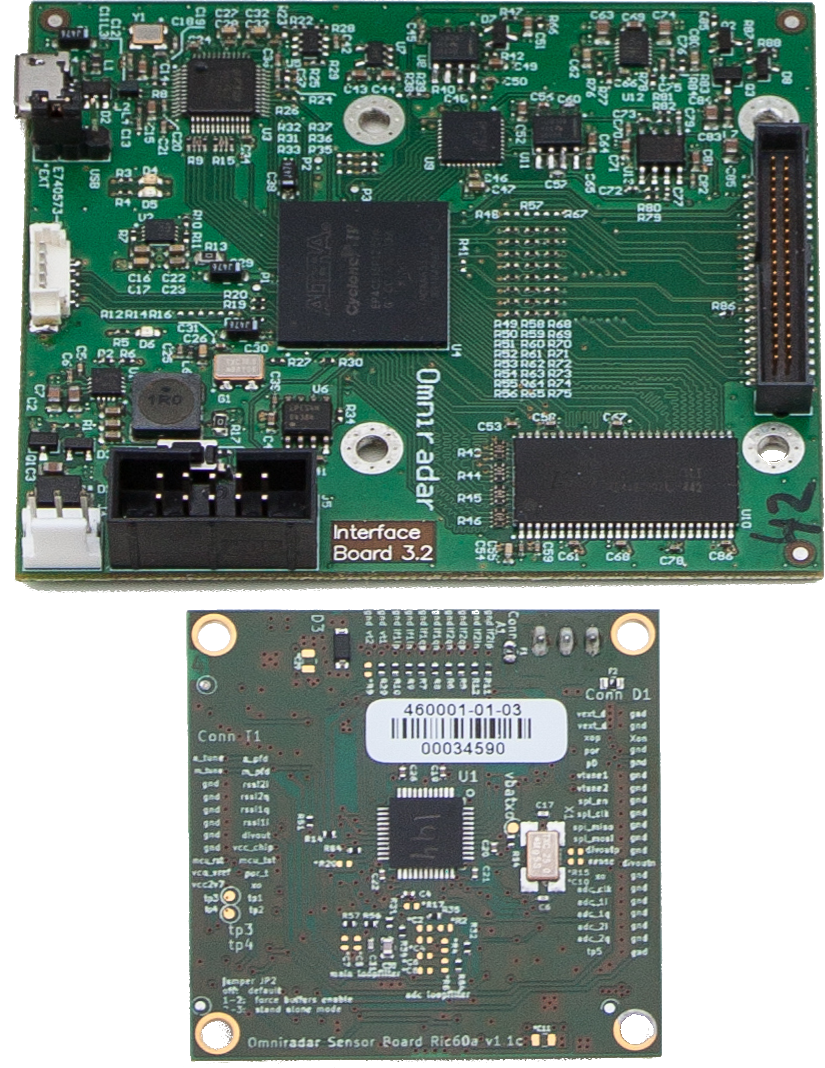
\includegraphics[max width=\hsize,max height=\maximheight,valign=t]{boards/img_omniradar}
\par\vspace{\extrarowheight}
\tabularnewline

Google / Infineon Soli\footnote{\url{https://www.infineon.com/cms/en/product/promopages/soli/}} &
Expected 2018. Sub-millimeter accuracy, running at over 10,000 frames per second \cite{Lien2016} &
\SI{60}{GHz}, \SI{7}{GHz} &
In\nobreakdash-package, 2~Tx,~4~Rx &
? &
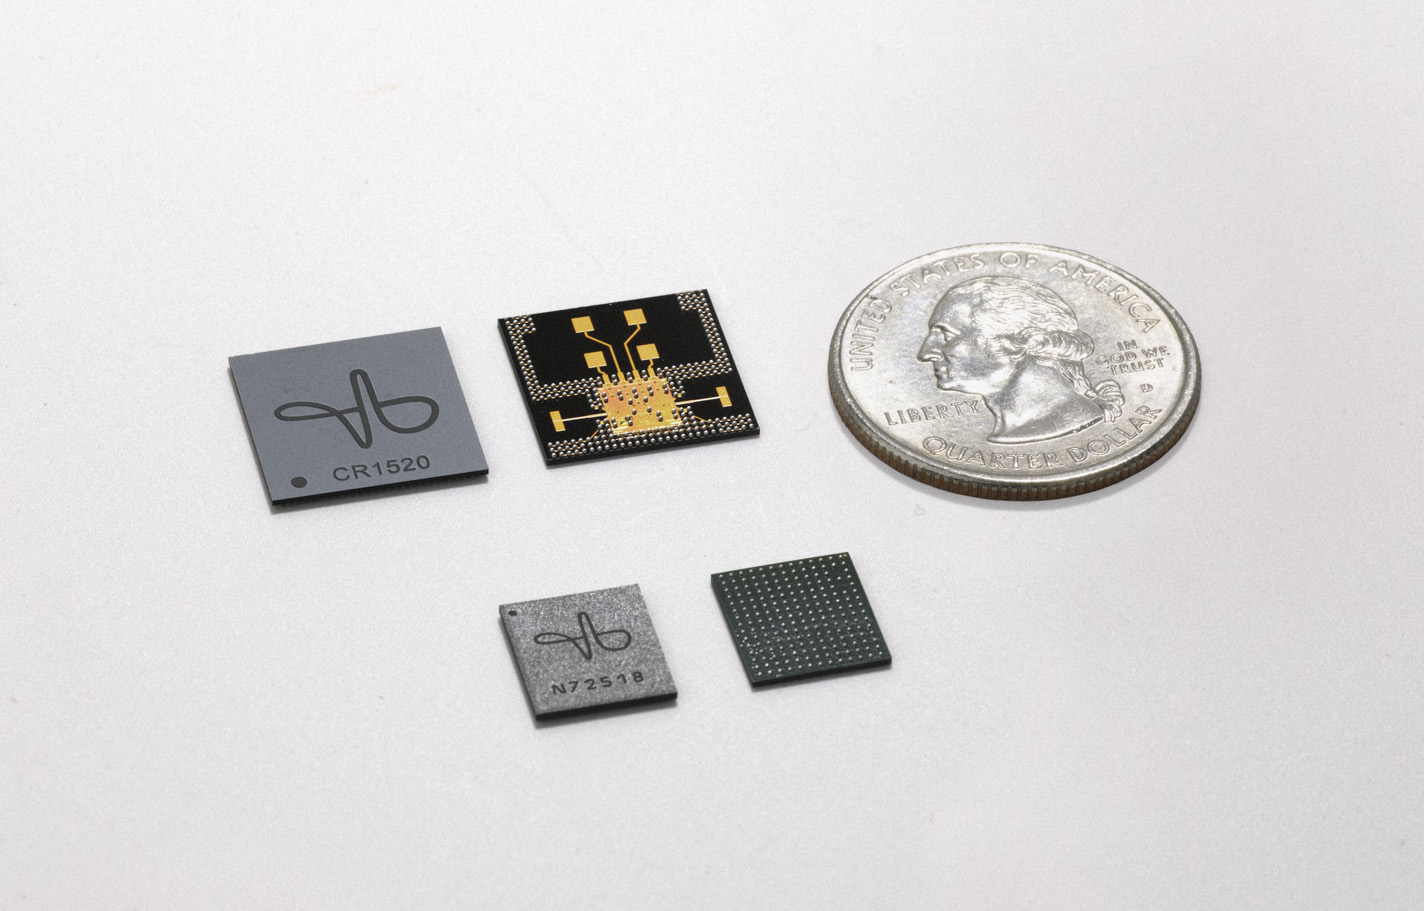
\includegraphics[max width=\hsize,max height=\maximheight,valign=t]{boards/img_soli.png}
\par\vspace{\extrarowheight}
\tabularnewline

Walabot Pro\footnote{\url{https://walabot.com/store/us/products/walabot-developer-pack.html}}&
3D configuration. Slow update rate&
\SI{6.8}{GHz}, \SI{7}{GHz} &
On\nobreakdash-board, 9~Tx,~9~Rx&
\$599&
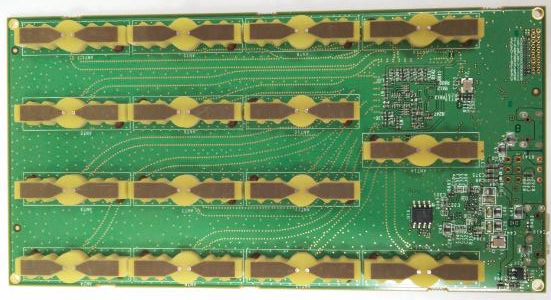
\includegraphics[max width=\hsize,max height=\maximheight,valign=t]{boards/img_walabot_1.png}
\par\vspace{\extrarowheight}
\tabularnewline

Bosch Prototype&
Two-port network analyzer used as core element in in-wall pipe detection&
\SI{5.15}{GHz}, \SI{6.7}{GHz} &
External, 2~Tx/Rx&
- &
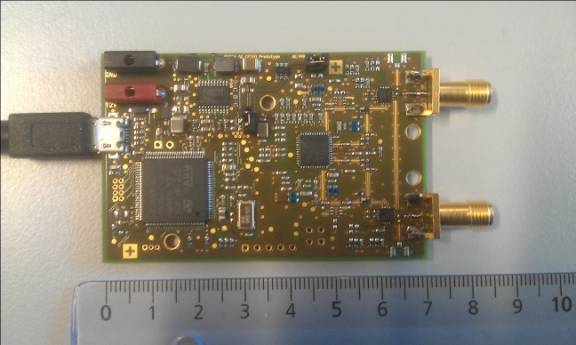
\includegraphics[max width=\hsize,max height=\maximheight,valign=t]{boards/img_bosch.jpg}
\par\vspace{\extrarowheight}
\tabularnewline

Silicon Radar SiRad Simple\footnote{\url{http://www.siliconradar.de/evalkits_e.html}}&
Has WiFi&
\SI{122}{GHz}, \SI{6.4}{GHz} &
On-chip, 1~Tx,~1~Rx&
?&
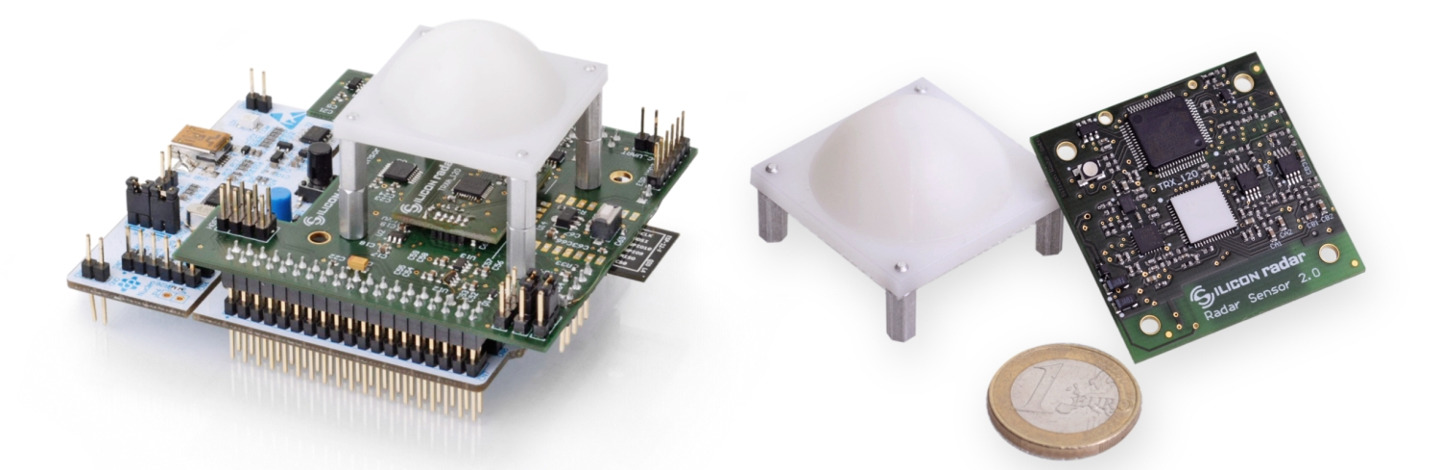
\includegraphics[max width=\hsize,max height=\maximheight,valign=t]{boards/img_silicon_radar.jpg}
\par\vspace{\extrarowheight}
\tabularnewline

Anokiwave AWMF-0117\footnote{\url{http://www.anokiwave.com/products/awmf-0117/index.html}}&
&
\SI{12.5}{GHz}, \SI{4.5}{GHz} &
On-chip, 1~Tx/Rx&
?&
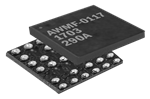
\includegraphics[max width=\hsize,max height=\maximheight,valign=t]{boards/img_anokiwave.png}
\par\vspace{\extrarowheight}
\tabularnewline

NXP Cocoon Radar\footnote{\url{Reuter2016}}&
Relatively small board. Presentation at FTF 2016 \cite{Reuter2016}&
\SI{77}{GHz}, \SI{4}{GHz} &
On\nobreakdash-board, 3~Tx,~4~Rx&
?&
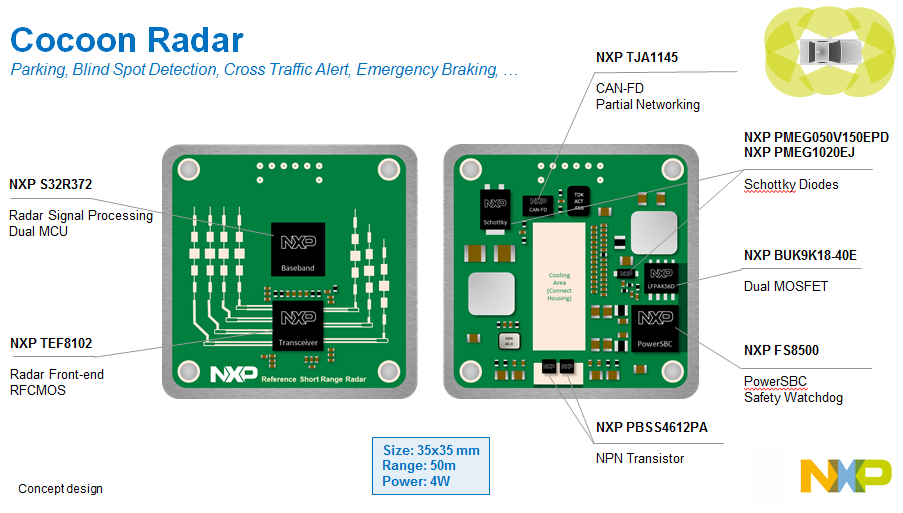
\includegraphics[max width=\hsize,max height=\maximheight,valign=t]{boards/img_cocoon.png}
\par\vspace{\extrarowheight}
\tabularnewline

TimeDomain P440\footnote{\url{http://www.timedomain.com/products/pulson-440/}}&
Can operate as multistatic radar or UWB communication node&
\SI{4}{GHz}, \SI{1.7}{GHz} &
External, 2~Tx/Rx&
\$5000&
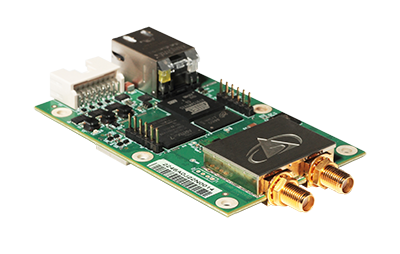
\includegraphics[max width=\hsize,max height=\maximheight,valign=t]{boards/img_p440.png}
\par\vspace{\extrarowheight}
\tabularnewline

Novelda Xethru X4M03\footnote{\url{https://www.xethru.com/xethru-development-platform.html}}&
&
\SI{8}{GHz}, \SI{1.5}{GHz} &
On\nobreakdash-board, 1~Tx/Rx&
\$399&
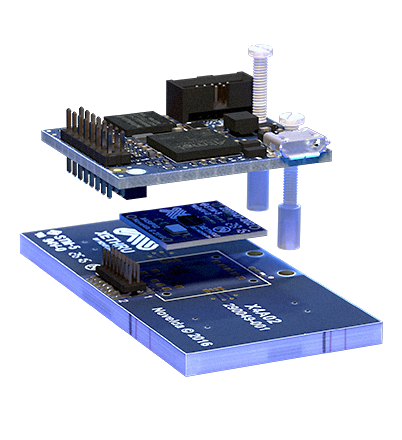
\includegraphics[max width=\hsize,max height=\maximheight,valign=t]{boards/img_xethru.png}
\par\vspace{\extrarowheight}
\tabularnewline

RFbeam MR2001\_RD\footnote{\url{https://www.rfbeam.ch/files/products/26/downloads/ProductBrief_MR2001_RD.pdf}}&
&
\SI{77}{GHz}, \SI{1}{GHz} &
On\nobreakdash-board, 4~Tx,~6~Rx&
?&
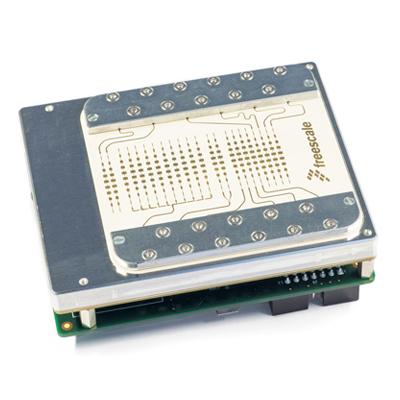
\includegraphics[max width=\hsize,max height=\maximheight,valign=t]{boards/img_rfbeam.jpg}
\par\vspace{\extrarowheight}
\tabularnewline

Inras \SI{77}{Ghz} Radarbook\footnote{\url{http://www.inras.at/en/products/radarbook.html}}&
Configurable FPGA processing chain&
\SI{77}{GHz}, \SI{1}{GHz} &
On\nobreakdash-board, 4~Tx,~8~Rx&
\$7300&
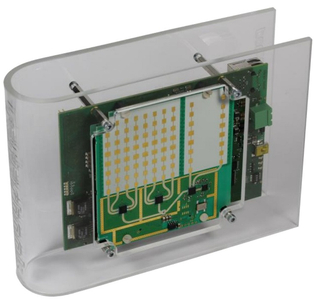
\includegraphics[max width=\hsize,max height=\maximheight,valign=t]{boards/img_radarbook.jpg}
\par\vspace{\extrarowheight}
\tabularnewline

Inras \SI{24}{Ghz} Radarbook\footnote{\url{dkradarbook}}&
&
\SI{24}{GHz}, \SI{250}{MHz} &
On\nobreakdash-board, 4~Tx,~4~Rx&
\$7300&
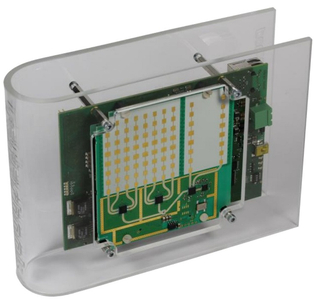
\includegraphics[max width=\hsize,max height=\maximheight,valign=t]{boards/img_radarbook.jpg}
\par\vspace{\extrarowheight}
\tabularnewline

Acconeer A1\footnote{\url{ http://www.acconeer.com/}}&
Sub-mm accuracy&
\SI{60}{GHz}, ? &
On-chip, ?&
?&
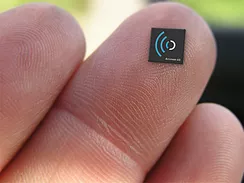
\includegraphics[max width=\hsize,max height=\maximheight,valign=t]{boards/img_acconeer.png}
\par\vspace{\extrarowheight}
\tabularnewline

Infineon BGT24-RFB2412-EVAL\footnote{\url{https://www.infineon.com/dgdl/?fileId=5546d46259d9a4bf0159f9f1fa503f1d}}&
&
\SI{24}{GHz}, \SI{250}{MHz} &
On\nobreakdash-board, 1~Tx,~2~Rx&
\$1333&
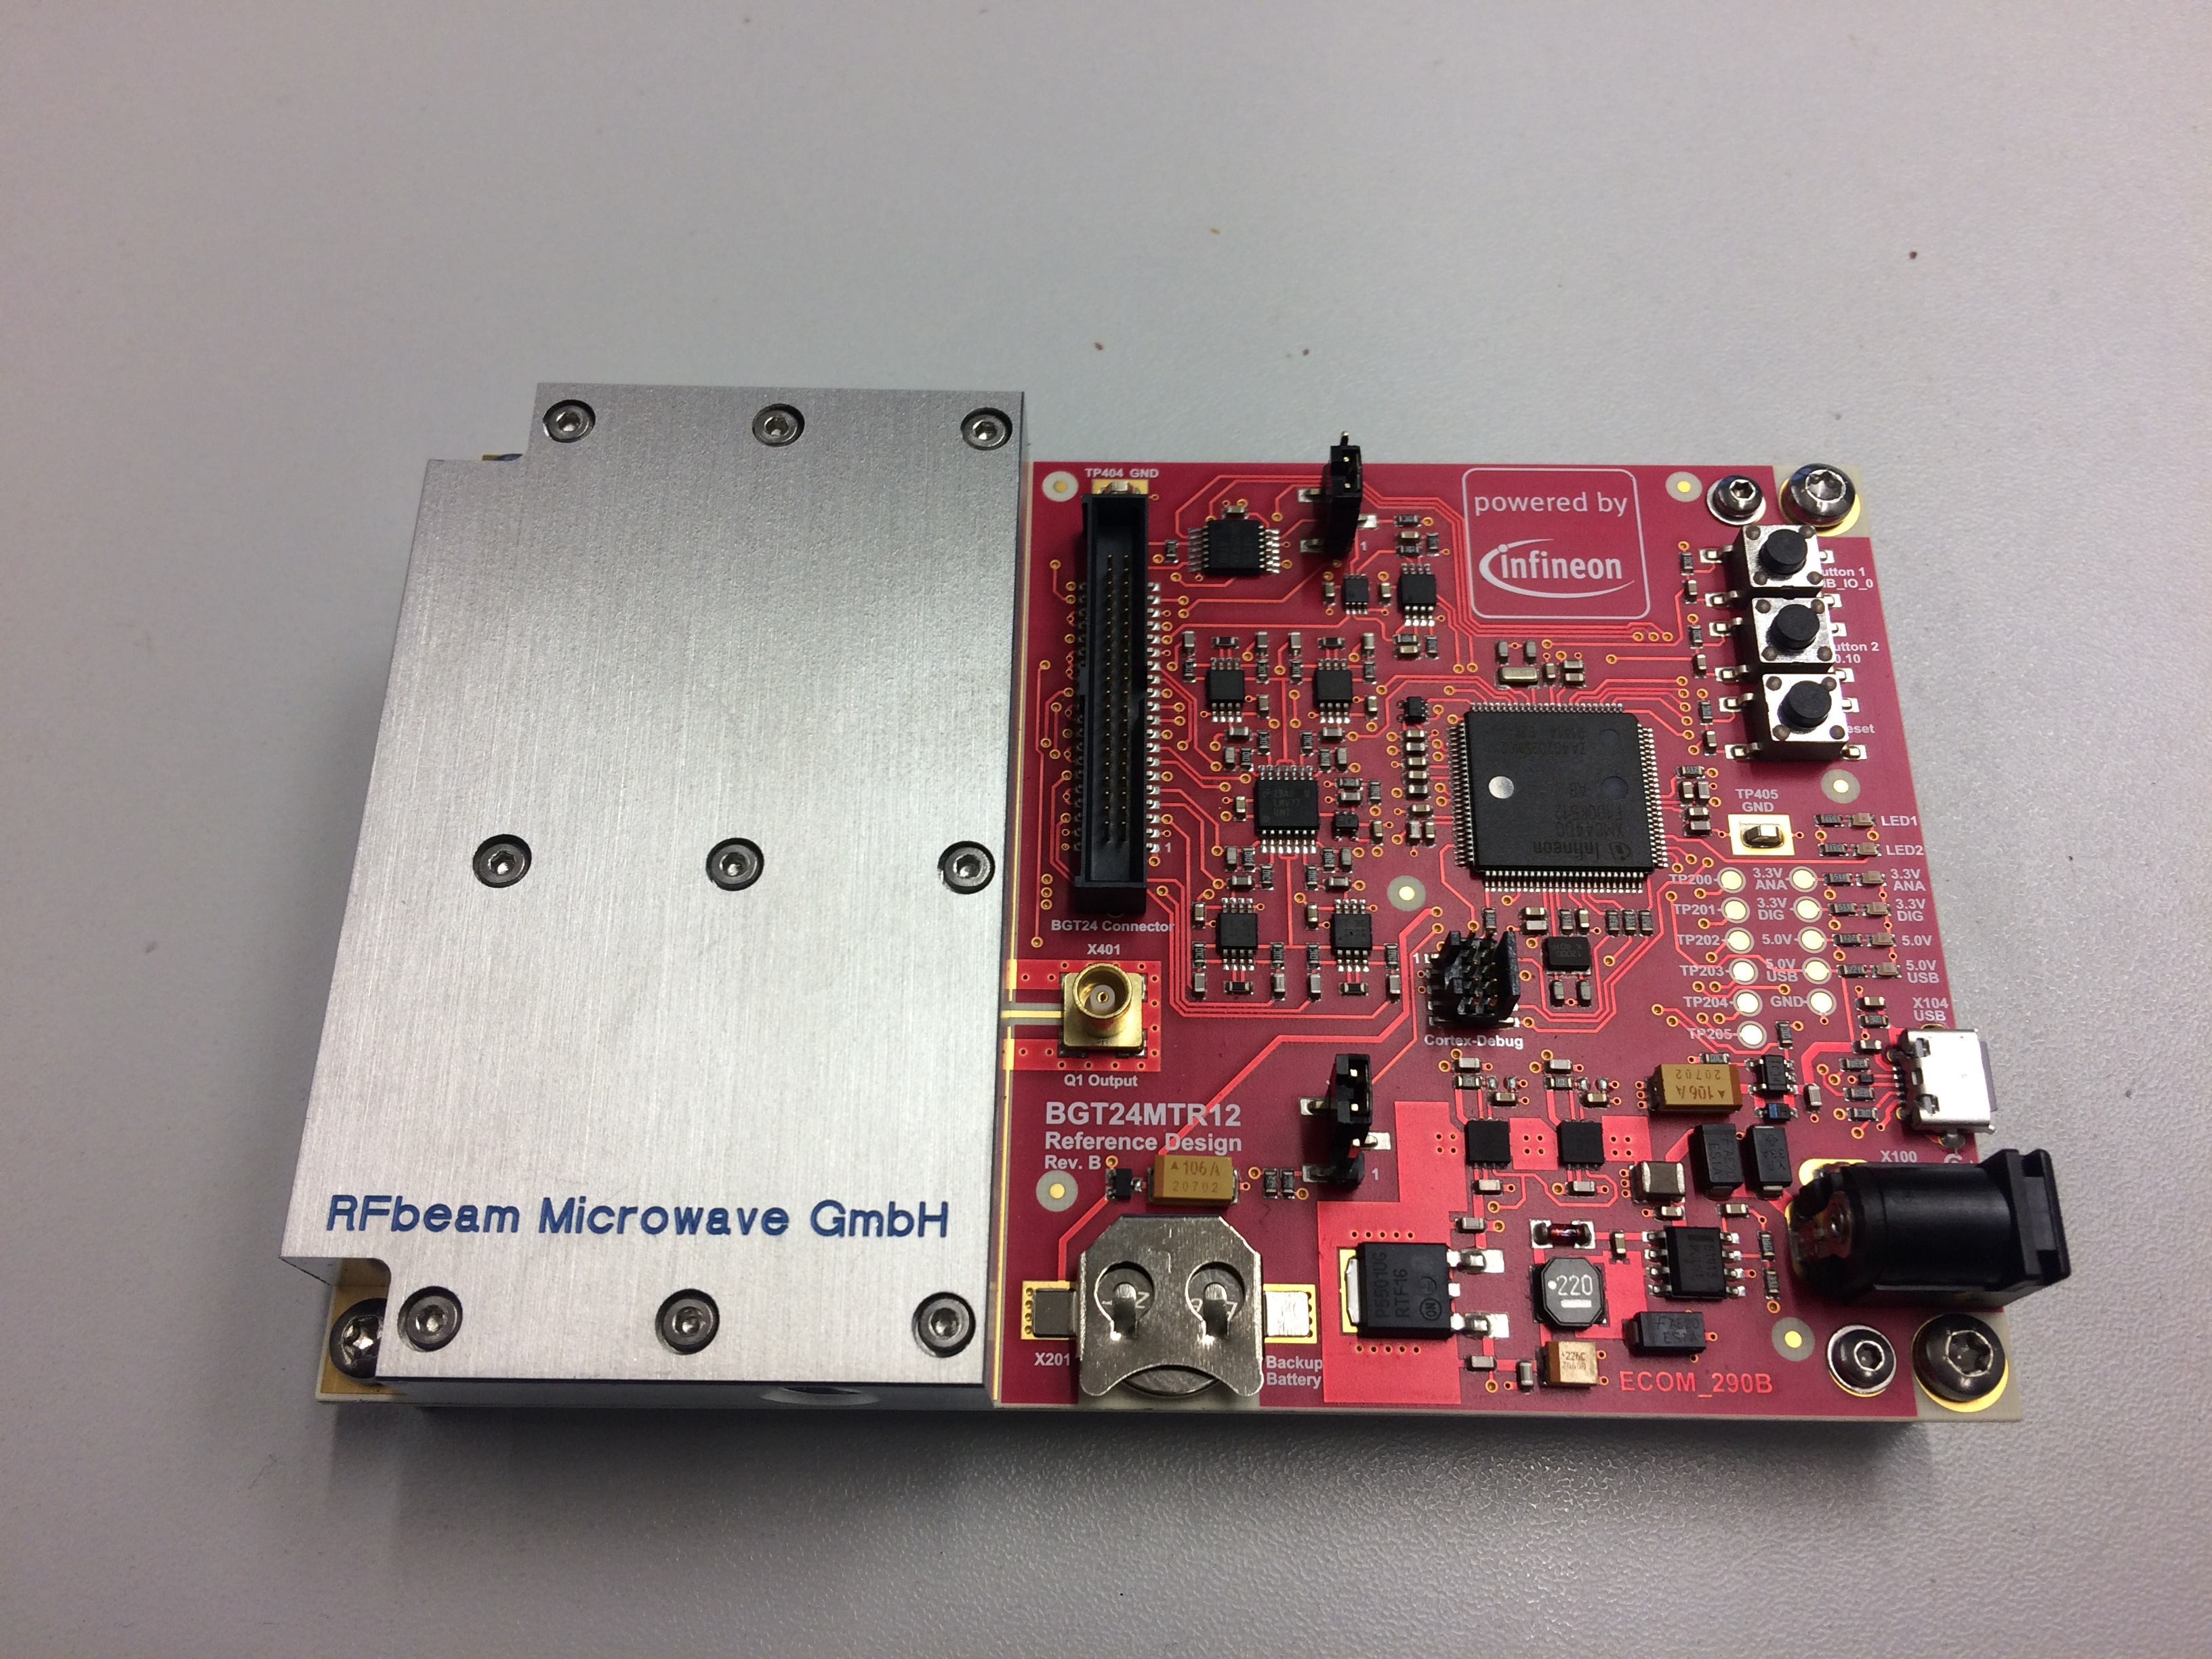
\includegraphics[max width=\hsize,max height=\maximheight,valign=t]{boards/img_bgt24.JPG}
\par\vspace{\extrarowheight}
\tabularnewline

IMST DK-sR-1200e\footnote{\url{http://webshop.imst.de/dk-sr-1200e-development-platform-for-24-ghz-fmcw-radar-application.html}}&
&
\SI{24}{GHz}, \SI{250}{MHz} &
On\nobreakdash-board, 1~Tx,~2~Rx&
\$3333&
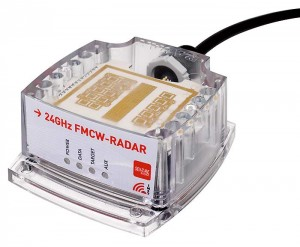
\includegraphics[max width=\hsize,max height=\maximheight,valign=t]{boards/img_IMST.jpg}
\par\vspace{\extrarowheight}
\tabularnewline

InnoSenT IVS-565\footnote{\url{http://www.innosent.de/fileadmin/media/dokumente/DATASHEETS_2016/Datenblatt_IVS-565.pdf}}&
&
\SI{24}{GHz}, \SI{250}{MHz} &
On\nobreakdash-board, 1~Tx,~2~Rx&
?&
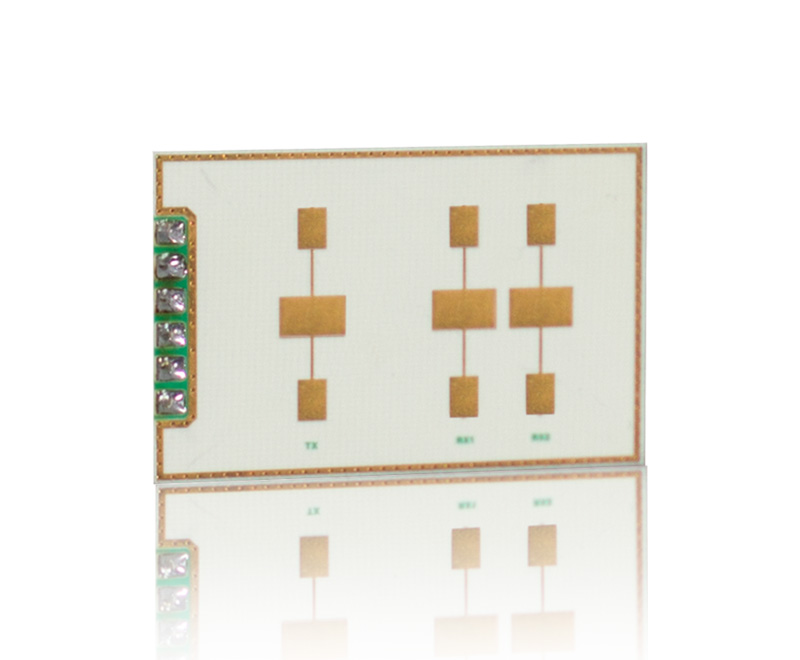
\includegraphics[max width=\hsize,max height=\maximheight,valign=t]{boards/img_innosent.jpg}
\par\vspace{\extrarowheight}
\tabularnewline

ST EVB-STradA431\footnote{\url{http://www.st.com/content/st_com/en/products/evaluation-tools/product-evaluation-tools/automotive-ic-eval-boards/evb-strada431.html}}&
SMA connectors for internal signals&
\SI{24}{GHz}, \SI{250}{MHz} &
External, 1~Tx,~3~Rx&
?&
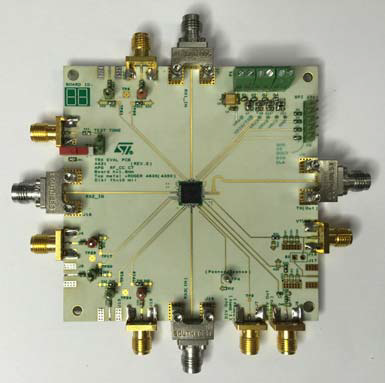
\includegraphics[max width=\hsize,max height=\maximheight,valign=t]{boards/img_ST.png}
\par\vspace{\extrarowheight}
\tabularnewline

OmniPreSense OPS241-A\footnote{\url{https://www.omnipresense.com/product/ops241-a/}}&
Arduino shield with BGT24LTR11&
\SI{24}{GHz}, \SI{80}{MHz} &
On\nobreakdash-board, 1~Tx/Rx&
\$169&
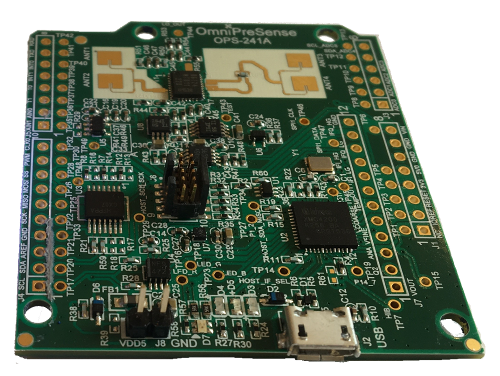
\includegraphics[max width=\hsize,max height=\maximheight,valign=t]{boards/img_omnipresense.png}
\par\vspace{\extrarowheight}
\tabularnewline

\bottomrule

\end{tabularx}

}
